\documentclass[11pt]{article}

\usepackage[spanish]{babel}

\usepackage[utf8]{inputenc}

\usepackage[T1]{fontenc}

\usepackage{amsmath}

\usepackage{booktabs}

\usepackage{graphicx}

\usepackage{float}

\usepackage{geometry}

\geometry{margin=2.4cm}

\title{Informe de resultados: Momentum general v1 plus}

\author{FinPUC}

\date{}

\begin{document}

\maketitle

\section{Analisis de resultados fuera de muestra}

La iteracion v1 plus conserva la probabilidad de abandono tipo umbral logistico y explicita una restriccion de ruina: cuando la riqueza actual del cliente llega a cero, el cliente abandona forzosamente la plataforma. La evaluacion fuera de muestra mantiene la separacion de horizontes y compara Black--Litterman calibrado contra Markowitz base en el Horizonte 3.

\begin{table}[H]
\centering
\resizebox{\textwidth}{!}{%
\begin{tabular}{lrrrrrrr}
\toprule
Escenario & Perfil & Sharpe BL & Sharpe MK & Mejora Sharpe & Drawdown BL & Drawdown MK & BL recomendado \\
\midrule
sin\_pandemia & Muy conservador & 1.760 & 1.736 & 1.4\% & -11.4\% & -10.3\% & 100.0\% \\
sin\_pandemia & Conservador & 1.760 & 1.728 & 1.8\% & -12.4\% & -11.0\% & 100.0\% \\
sin\_pandemia & Neutro & 1.582 & 1.747 & -9.4\% & -15.9\% & -13.0\% & 0.0\% \\
sin\_pandemia & Arriesgado & 1.040 & 1.513 & -31.2\% & -29.0\% & -18.2\% & 0.0\% \\
sin\_pandemia & Muy arriesgado & 0.579 & 1.198 & -51.6\% & -41.1\% & -26.5\% & 0.0\% \\
con\_pandemia & Muy conservador & 1.889 & 1.699 & 11.3\% & -9.6\% & -9.0\% & 100.0\% \\
con\_pandemia & Conservador & 2.140 & 1.749 & 22.5\% & -9.7\% & -9.0\% & 100.0\% \\
con\_pandemia & Neutro & 1.937 & 1.773 & 9.2\% & -15.5\% & -10.9\% & 0.0\% \\
con\_pandemia & Arriesgado & 1.702 & 1.391 & 22.2\% & -27.9\% & -18.7\% & 0.0\% \\
con\_pandemia & Muy arriesgado & 1.634 & 0.933 & 75.6\% & -40.9\% & -27.6\% & 0.0\% \\
\bottomrule
\end{tabular}
}
\caption{Comparacion fuera de muestra para Momentum general.}
\label{tab:test_momentum_general_v1_plus}
\end{table}


\section{Resultados de la dinamica de portafolio}

La dinamica del portafolio se interpreta desde la estabilidad operativa. Turnover bajo indica menor intensidad de transaccion semestral; HHI y peso del sector dominante permiten identificar si el desempeno proviene de una exposicion diversificada o de apuestas concentradas.

\begin{table}[H]
\centering
\resizebox{\textwidth}{!}{%
\begin{tabular}{lrrrrrrr}
\toprule
Modelo & Escenario & Perfil & Turnover & Turnover max. & N efectivo & HHI sector & Sector top \\
\midrule
BL calibrado & sin\_pandemia & Muy conservador & 13.4\% & 15.8\% & 231.32 & 0.158 & 30.6\% \\
Markowitz base & sin\_pandemia & Muy conservador & 5.6\% & 6.4\% & 203.23 & 0.151 & 28.4\% \\
BL calibrado & sin\_pandemia & Conservador & 21.4\% & 26.3\% & 223.36 & 0.168 & 32.4\% \\
Markowitz base & sin\_pandemia & Conservador & 5.8\% & 7.2\% & 194.60 & 0.150 & 28.7\% \\
BL calibrado & sin\_pandemia & Neutro & 42.2\% & 50.2\% & 128.81 & 0.209 & 38.7\% \\
Markowitz base & sin\_pandemia & Neutro & 8.1\% & 10.0\% & 148.30 & 0.152 & 29.3\% \\
BL calibrado & sin\_pandemia & Arriesgado & 59.6\% & 74.9\% & 39.73 & 0.293 & 47.5\% \\
Markowitz base & sin\_pandemia & Arriesgado & 12.4\% & 13.2\% & 64.35 & 0.184 & 30.5\% \\
BL calibrado & sin\_pandemia & Muy arriesgado & 60.0\% & 91.0\% & 17.44 & 0.303 & 41.8\% \\
Markowitz base & sin\_pandemia & Muy arriesgado & 13.0\% & 13.9\% & 19.72 & 0.273 & 43.2\% \\
BL calibrado & con\_pandemia & Muy conservador & 12.7\% & 17.0\% & 113.14 & 0.175 & 28.2\% \\
Markowitz base & con\_pandemia & Muy conservador & 5.0\% & 6.6\% & 106.76 & 0.164 & 24.9\% \\
BL calibrado & con\_pandemia & Conservador & 22.1\% & 28.7\% & 107.93 & 0.177 & 29.3\% \\
Markowitz base & con\_pandemia & Conservador & 5.9\% & 7.7\% & 107.08 & 0.156 & 23.6\% \\
BL calibrado & con\_pandemia & Neutro & 33.3\% & 46.5\% & 57.36 & 0.224 & 38.5\% \\
Markowitz base & con\_pandemia & Neutro & 8.4\% & 10.7\% & 89.27 & 0.144 & 22.5\% \\
BL calibrado & con\_pandemia & Arriesgado & 42.1\% & 69.4\% & 16.57 & 0.352 & 52.7\% \\
Markowitz base & con\_pandemia & Arriesgado & 13.4\% & 17.7\% & 42.73 & 0.182 & 26.9\% \\
BL calibrado & con\_pandemia & Muy arriesgado & 39.7\% & 70.0\% & 6.43 & 0.545 & 67.9\% \\
Markowitz base & con\_pandemia & Muy arriesgado & 14.1\% & 18.2\% & 13.97 & 0.243 & 40.1\% \\
\bottomrule
\end{tabular}
}
\caption{Dinamica de portafolio para Momentum general.}
\label{tab:dinamica_momentum_general_v1_plus}
\end{table}


\section{Evaluacion Economica Monte Carlo P4 en Horizonte Limpio}

En la view Momentum general, la lectura economica del Horizonte 3 se realiza sin retroalimentar la utilidad de empresa al optimizador. El mayor score P4 promedio dentro de Black--Litterman se observa en el perfil Muy arriesgado bajo escenario con\_pandemia, mientras que la mayor presion mensual de abandono aparece en Muy conservador bajo sin\_pandemia. Esta distincion es central: la recomendacion financiera se evalua por desempeno y estabilidad del portafolio, y la utilidad corporativa queda como consecuencia ex-post del saldo administrado que permanece activo.

\begin{table}[H]
\centering
\resizebox{\textwidth}{!}{%
\begin{tabular}{lrrrrrrrr}
\toprule
Modelo & Escenario & Perfil & Riqueza & Utilidad empresa & P acepta reb. & P abandono sem. & P abandono mes & Clientes finales \\
\midrule
BL calibrado & sin\_pandemia & Muy conservador & 1.457 & 127 & 55.8\% & 0.6\% & 1.3\% & 431 \\
Markowitz base & sin\_pandemia & Muy conservador & 1.390 & 116 & 55.7\% & 0.6\% & 1.2\% & 412 \\
BL calibrado & sin\_pandemia & Conservador & 1.977 & 267 & 54.8\% & 0.1\% & 0.2\% & 946 \\
Markowitz base & sin\_pandemia & Conservador & 1.856 & 248 & 54.4\% & 0.1\% & 0.3\% & 910 \\
BL calibrado & sin\_pandemia & Neutro & 2.274 & 312 & 53.0\% & 0.0\% & 0.0\% & 1041 \\
Markowitz base & sin\_pandemia & Neutro & 2.043 & 283 & 52.5\% & 0.0\% & 0.0\% & 1028 \\
BL calibrado & sin\_pandemia & Arriesgado & 2.291 & 305 & 49.6\% & 0.0\% & 0.1\% & 954 \\
Markowitz base & sin\_pandemia & Arriesgado & 2.255 & 299 & 49.7\% & 0.0\% & 0.0\% & 986 \\
Markowitz base & sin\_pandemia & Muy arriesgado & 2.701 & 344 & 48.6\% & 0.0\% & 0.0\% & 990 \\
BL calibrado & sin\_pandemia & Muy arriesgado & 1.641 & 209 & 45.4\% & 0.1\% & 0.4\% & 703 \\
BL calibrado & con\_pandemia & Muy conservador & 1.457 & 127 & 55.9\% & 0.5\% & 1.2\% & 445 \\
Markowitz base & con\_pandemia & Muy conservador & 1.338 & 109 & 55.1\% & 0.6\% & 1.2\% & 412 \\
BL calibrado & con\_pandemia & Conservador & 2.291 & 304 & 55.9\% & 0.1\% & 0.2\% & 978 \\
Markowitz base & con\_pandemia & Conservador & 1.776 & 243 & 54.0\% & 0.1\% & 0.2\% & 943 \\
BL calibrado & con\_pandemia & Neutro & 3.311 & 419 & 55.9\% & 0.0\% & 0.1\% & 1075 \\
Markowitz base & con\_pandemia & Neutro & 1.995 & 280 & 52.2\% & 0.0\% & 0.0\% & 1035 \\
BL calibrado & con\_pandemia & Arriesgado & 6.847 & 715 & 57.1\% & 0.0\% & 0.1\% & 1075 \\
Markowitz base & con\_pandemia & Arriesgado & 2.198 & 289 & 49.5\% & 0.0\% & 0.0\% & 964 \\
BL calibrado & con\_pandemia & Muy arriesgado & 15.983 & 1.338 & 59.8\% & 0.0\% & 0.2\% & 1067 \\
Markowitz base & con\_pandemia & Muy arriesgado & 2.330 & 297 & 47.6\% & 0.0\% & 0.1\% & 894 \\
\bottomrule
\end{tabular}
}
\caption{Resultados economicos P4 con restriccion de ruina para Momentum general.}
\label{tab:p4_momentum_general_v1_plus}
\end{table}


\begin{table}[H]
\centering
\resizebox{\textwidth}{!}{%
\begin{tabular}{lrrrrrrrr}
\toprule
Modelo & Escenario & Perfil & P inicial & P reb. & P sem. & P mes & Clientes iniciales & Clientes finales \\
\midrule
BL calibrado & sin\_pandemia & Muy conservador & 55.8\% & 55.8\% & 0.6\% & 1.3\% & 1123 & 431 \\
Markowitz base & sin\_pandemia & Muy conservador & 55.7\% & 55.7\% & 0.6\% & 1.2\% & 1085 & 412 \\
BL calibrado & sin\_pandemia & Conservador & 54.8\% & 54.8\% & 0.1\% & 0.2\% & 1102 & 946 \\
Markowitz base & sin\_pandemia & Conservador & 54.4\% & 54.4\% & 0.1\% & 0.3\% & 1088 & 910 \\
BL calibrado & sin\_pandemia & Neutro & 53.0\% & 53.0\% & 0.0\% & 0.0\% & 1073 & 1041 \\
Markowitz base & sin\_pandemia & Neutro & 52.5\% & 52.5\% & 0.0\% & 0.0\% & 1039 & 1028 \\
BL calibrado & sin\_pandemia & Arriesgado & 49.6\% & 49.6\% & 0.0\% & 0.1\% & 1022 & 954 \\
Markowitz base & sin\_pandemia & Arriesgado & 49.7\% & 49.7\% & 0.0\% & 0.0\% & 988 & 986 \\
BL calibrado & sin\_pandemia & Muy arriesgado & 45.4\% & 45.4\% & 0.1\% & 0.4\% & 895 & 703 \\
Markowitz base & sin\_pandemia & Muy arriesgado & 48.6\% & 48.6\% & 0.0\% & 0.0\% & 1009 & 990 \\
BL calibrado & con\_pandemia & Muy conservador & 55.9\% & 55.9\% & 0.5\% & 1.2\% & 1100 & 445 \\
Markowitz base & con\_pandemia & Muy conservador & 55.1\% & 55.1\% & 0.6\% & 1.2\% & 1103 & 412 \\
BL calibrado & con\_pandemia & Conservador & 55.9\% & 55.9\% & 0.1\% & 0.2\% & 1124 & 978 \\
Markowitz base & con\_pandemia & Conservador & 54.0\% & 54.0\% & 0.1\% & 0.2\% & 1088 & 943 \\
BL calibrado & con\_pandemia & Neutro & 55.9\% & 55.9\% & 0.0\% & 0.1\% & 1118 & 1075 \\
Markowitz base & con\_pandemia & Neutro & 52.2\% & 52.2\% & 0.0\% & 0.0\% & 1040 & 1035 \\
BL calibrado & con\_pandemia & Arriesgado & 57.1\% & 57.1\% & 0.0\% & 0.1\% & 1134 & 1075 \\
Markowitz base & con\_pandemia & Arriesgado & 49.5\% & 49.5\% & 0.0\% & 0.0\% & 970 & 964 \\
BL calibrado & con\_pandemia & Muy arriesgado & 59.8\% & 59.8\% & 0.0\% & 0.2\% & 1181 & 1067 \\
Markowitz base & con\_pandemia & Muy arriesgado & 47.6\% & 47.6\% & 0.0\% & 0.1\% & 956 & 894 \\
\bottomrule
\end{tabular}
}
\caption{Probabilidades de comportamiento y clientes activos para Momentum general.}
\label{tab:behavior_momentum_general_v1_plus}
\end{table}


\subsection{Trayectorias semanales y mensuales}

\begin{figure}[H]
\centering

\includegraphics[width=0.92\textwidth]{figuras/clientes_weekly_sin_pandemia_bl_calibrado.png}
\caption{Clientes activos semanales por perfil, BL calibrado, escenario sin pandemia.}
\label{fig:clientes_weekly_momentum_general_v1_plus_sin_pandemia_bl_calibrado}
\end{figure}


\begin{figure}[H]
\centering

\includegraphics[width=0.92\textwidth]{figuras/abandono_weekly_sin_pandemia_bl_calibrado.png}
\caption{Probabilidad semanal de abandono por perfil, BL calibrado, escenario sin pandemia.}
\label{fig:abandono_weekly_momentum_general_v1_plus_sin_pandemia_bl_calibrado}
\end{figure}


\begin{figure}[H]
\centering

\includegraphics[width=0.92\textwidth]{figuras/aceptacion_weekly_sin_pandemia_bl_calibrado.png}
\caption{Probabilidad semanal de aceptacion de rebalanceo por perfil, BL calibrado, escenario sin pandemia.}
\label{fig:aceptacion_weekly_momentum_general_v1_plus_sin_pandemia_bl_calibrado}
\end{figure}


\begin{figure}[H]
\centering

\includegraphics[width=0.92\textwidth]{figuras/ganancia_weekly_sin_pandemia_bl_calibrado.png}
\caption{Ganancia semanal promedio por perfil, BL calibrado, escenario sin pandemia.}
\label{fig:ganancia_weekly_momentum_general_v1_plus_sin_pandemia_bl_calibrado}
\end{figure}


\begin{figure}[H]
\centering

\includegraphics[width=0.92\textwidth]{figuras/clientes_monthly_sin_pandemia_bl_calibrado.png}
\caption{Clientes activos mensuales por perfil, BL calibrado, escenario sin pandemia.}
\label{fig:clientes_monthly_momentum_general_v1_plus_sin_pandemia_bl_calibrado}
\end{figure}


\begin{figure}[H]
\centering

\includegraphics[width=0.92\textwidth]{figuras/abandono_monthly_sin_pandemia_bl_calibrado.png}
\caption{Probabilidad mensual de abandono por perfil, BL calibrado, escenario sin pandemia.}
\label{fig:abandono_monthly_momentum_general_v1_plus_sin_pandemia_bl_calibrado}
\end{figure}


\begin{figure}[H]
\centering

\includegraphics[width=0.92\textwidth]{figuras/aceptacion_monthly_sin_pandemia_bl_calibrado.png}
\caption{Probabilidad mensual de aceptacion de rebalanceo por perfil, BL calibrado, escenario sin pandemia.}
\label{fig:aceptacion_monthly_momentum_general_v1_plus_sin_pandemia_bl_calibrado}
\end{figure}


\begin{figure}[H]
\centering

\includegraphics[width=0.92\textwidth]{figuras/ganancia_monthly_sin_pandemia_bl_calibrado.png}
\caption{Ganancia mensual promedio por perfil, BL calibrado, escenario sin pandemia.}
\label{fig:ganancia_monthly_momentum_general_v1_plus_sin_pandemia_bl_calibrado}
\end{figure}


\begin{figure}[H]
\centering

\includegraphics[width=0.92\textwidth]{figuras/ganancia_semiannual_sin_pandemia_bl_calibrado.png}
\caption{Ganancia semestral promedio por perfil, BL calibrado, escenario sin pandemia.}
\label{fig:ganancia_semiannual_momentum_general_v1_plus_sin_pandemia_bl_calibrado}
\end{figure}


\begin{figure}[H]
\centering

\includegraphics[width=0.92\textwidth]{figuras/clientes_weekly_sin_pandemia_markowitz_base.png}
\caption{Clientes activos semanales por perfil, Markowitz base, escenario sin pandemia.}
\label{fig:clientes_weekly_momentum_general_v1_plus_sin_pandemia_markowitz_base}
\end{figure}


\begin{figure}[H]
\centering

\includegraphics[width=0.92\textwidth]{figuras/abandono_weekly_sin_pandemia_markowitz_base.png}
\caption{Probabilidad semanal de abandono por perfil, Markowitz base, escenario sin pandemia.}
\label{fig:abandono_weekly_momentum_general_v1_plus_sin_pandemia_markowitz_base}
\end{figure}


\begin{figure}[H]
\centering
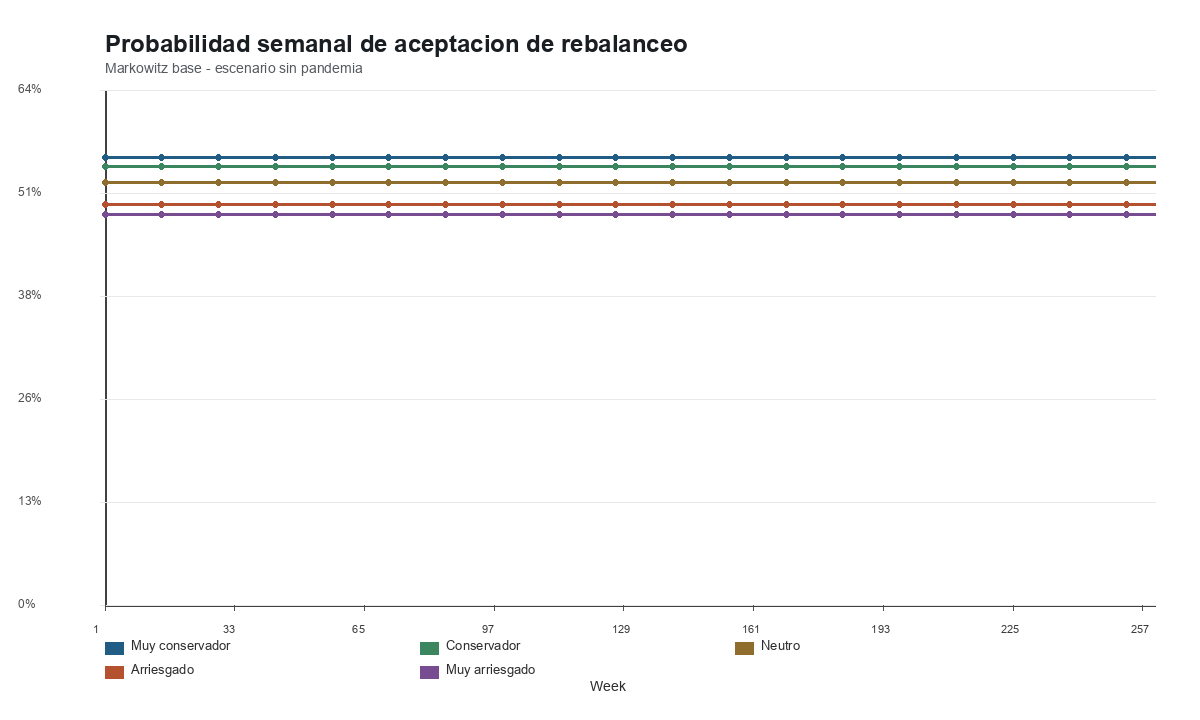
\includegraphics[width=0.92\textwidth]{figuras/aceptacion_weekly_sin_pandemia_markowitz_base.png}
\caption{Probabilidad semanal de aceptacion de rebalanceo por perfil, Markowitz base, escenario sin pandemia.}
\label{fig:aceptacion_weekly_momentum_general_v1_plus_sin_pandemia_markowitz_base}
\end{figure}


\begin{figure}[H]
\centering

\includegraphics[width=0.92\textwidth]{figuras/ganancia_weekly_sin_pandemia_markowitz_base.png}
\caption{Ganancia semanal promedio por perfil, Markowitz base, escenario sin pandemia.}
\label{fig:ganancia_weekly_momentum_general_v1_plus_sin_pandemia_markowitz_base}
\end{figure}


\begin{figure}[H]
\centering

\includegraphics[width=0.92\textwidth]{figuras/clientes_monthly_sin_pandemia_markowitz_base.png}
\caption{Clientes activos mensuales por perfil, Markowitz base, escenario sin pandemia.}
\label{fig:clientes_monthly_momentum_general_v1_plus_sin_pandemia_markowitz_base}
\end{figure}


\begin{figure}[H]
\centering

\includegraphics[width=0.92\textwidth]{figuras/abandono_monthly_sin_pandemia_markowitz_base.png}
\caption{Probabilidad mensual de abandono por perfil, Markowitz base, escenario sin pandemia.}
\label{fig:abandono_monthly_momentum_general_v1_plus_sin_pandemia_markowitz_base}
\end{figure}


\begin{figure}[H]
\centering
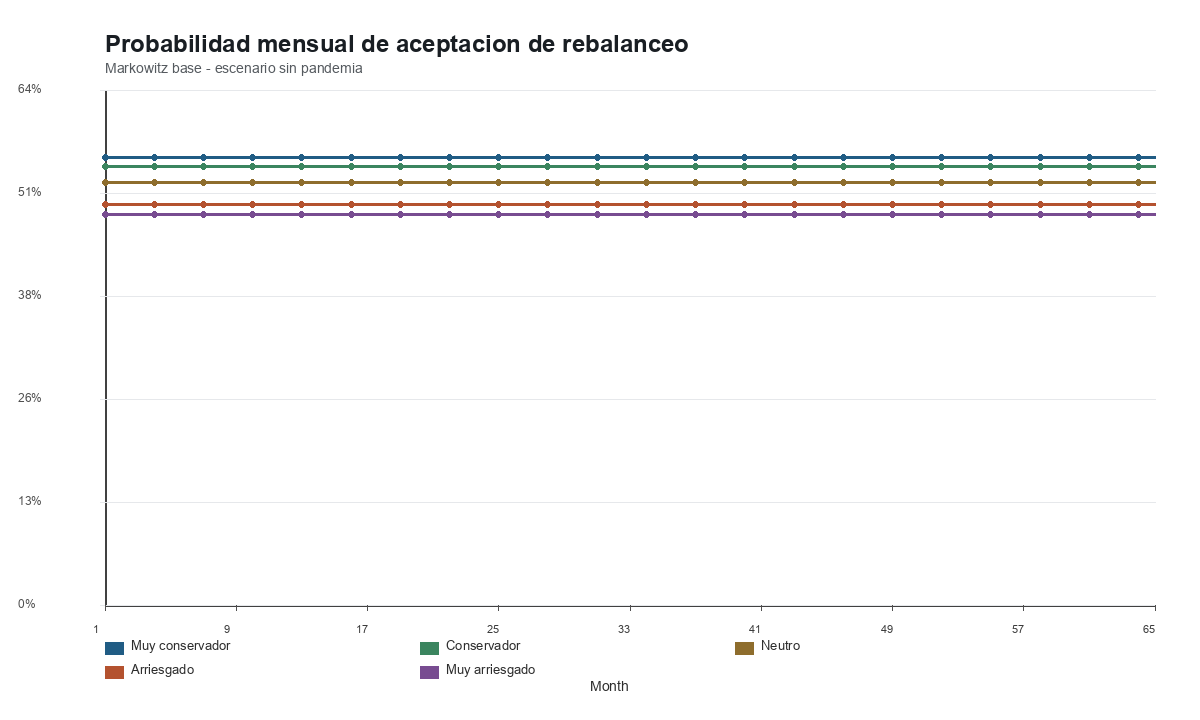
\includegraphics[width=0.92\textwidth]{figuras/aceptacion_monthly_sin_pandemia_markowitz_base.png}
\caption{Probabilidad mensual de aceptacion de rebalanceo por perfil, Markowitz base, escenario sin pandemia.}
\label{fig:aceptacion_monthly_momentum_general_v1_plus_sin_pandemia_markowitz_base}
\end{figure}


\begin{figure}[H]
\centering

\includegraphics[width=0.92\textwidth]{figuras/ganancia_monthly_sin_pandemia_markowitz_base.png}
\caption{Ganancia mensual promedio por perfil, Markowitz base, escenario sin pandemia.}
\label{fig:ganancia_monthly_momentum_general_v1_plus_sin_pandemia_markowitz_base}
\end{figure}


\begin{figure}[H]
\centering

\includegraphics[width=0.92\textwidth]{figuras/ganancia_semiannual_sin_pandemia_markowitz_base.png}
\caption{Ganancia semestral promedio por perfil, Markowitz base, escenario sin pandemia.}
\label{fig:ganancia_semiannual_momentum_general_v1_plus_sin_pandemia_markowitz_base}
\end{figure}


\begin{figure}[H]
\centering

\includegraphics[width=0.92\textwidth]{figuras/clientes_weekly_con_pandemia_bl_calibrado.png}
\caption{Clientes activos semanales por perfil, BL calibrado, escenario con pandemia.}
\label{fig:clientes_weekly_momentum_general_v1_plus_con_pandemia_bl_calibrado}
\end{figure}


\begin{figure}[H]
\centering

\includegraphics[width=0.92\textwidth]{figuras/abandono_weekly_con_pandemia_bl_calibrado.png}
\caption{Probabilidad semanal de abandono por perfil, BL calibrado, escenario con pandemia.}
\label{fig:abandono_weekly_momentum_general_v1_plus_con_pandemia_bl_calibrado}
\end{figure}


\begin{figure}[H]
\centering

\includegraphics[width=0.92\textwidth]{figuras/aceptacion_weekly_con_pandemia_bl_calibrado.png}
\caption{Probabilidad semanal de aceptacion de rebalanceo por perfil, BL calibrado, escenario con pandemia.}
\label{fig:aceptacion_weekly_momentum_general_v1_plus_con_pandemia_bl_calibrado}
\end{figure}


\begin{figure}[H]
\centering

\includegraphics[width=0.92\textwidth]{figuras/ganancia_weekly_con_pandemia_bl_calibrado.png}
\caption{Ganancia semanal promedio por perfil, BL calibrado, escenario con pandemia.}
\label{fig:ganancia_weekly_momentum_general_v1_plus_con_pandemia_bl_calibrado}
\end{figure}


\begin{figure}[H]
\centering

\includegraphics[width=0.92\textwidth]{figuras/clientes_monthly_con_pandemia_bl_calibrado.png}
\caption{Clientes activos mensuales por perfil, BL calibrado, escenario con pandemia.}
\label{fig:clientes_monthly_momentum_general_v1_plus_con_pandemia_bl_calibrado}
\end{figure}


\begin{figure}[H]
\centering

\includegraphics[width=0.92\textwidth]{figuras/abandono_monthly_con_pandemia_bl_calibrado.png}
\caption{Probabilidad mensual de abandono por perfil, BL calibrado, escenario con pandemia.}
\label{fig:abandono_monthly_momentum_general_v1_plus_con_pandemia_bl_calibrado}
\end{figure}


\begin{figure}[H]
\centering

\includegraphics[width=0.92\textwidth]{figuras/aceptacion_monthly_con_pandemia_bl_calibrado.png}
\caption{Probabilidad mensual de aceptacion de rebalanceo por perfil, BL calibrado, escenario con pandemia.}
\label{fig:aceptacion_monthly_momentum_general_v1_plus_con_pandemia_bl_calibrado}
\end{figure}


\begin{figure}[H]
\centering

\includegraphics[width=0.92\textwidth]{figuras/ganancia_monthly_con_pandemia_bl_calibrado.png}
\caption{Ganancia mensual promedio por perfil, BL calibrado, escenario con pandemia.}
\label{fig:ganancia_monthly_momentum_general_v1_plus_con_pandemia_bl_calibrado}
\end{figure}


\begin{figure}[H]
\centering

\includegraphics[width=0.92\textwidth]{figuras/ganancia_semiannual_con_pandemia_bl_calibrado.png}
\caption{Ganancia semestral promedio por perfil, BL calibrado, escenario con pandemia.}
\label{fig:ganancia_semiannual_momentum_general_v1_plus_con_pandemia_bl_calibrado}
\end{figure}


\begin{figure}[H]
\centering

\includegraphics[width=0.92\textwidth]{figuras/clientes_weekly_con_pandemia_markowitz_base.png}
\caption{Clientes activos semanales por perfil, Markowitz base, escenario con pandemia.}
\label{fig:clientes_weekly_momentum_general_v1_plus_con_pandemia_markowitz_base}
\end{figure}


\begin{figure}[H]
\centering

\includegraphics[width=0.92\textwidth]{figuras/abandono_weekly_con_pandemia_markowitz_base.png}
\caption{Probabilidad semanal de abandono por perfil, Markowitz base, escenario con pandemia.}
\label{fig:abandono_weekly_momentum_general_v1_plus_con_pandemia_markowitz_base}
\end{figure}


\begin{figure}[H]
\centering
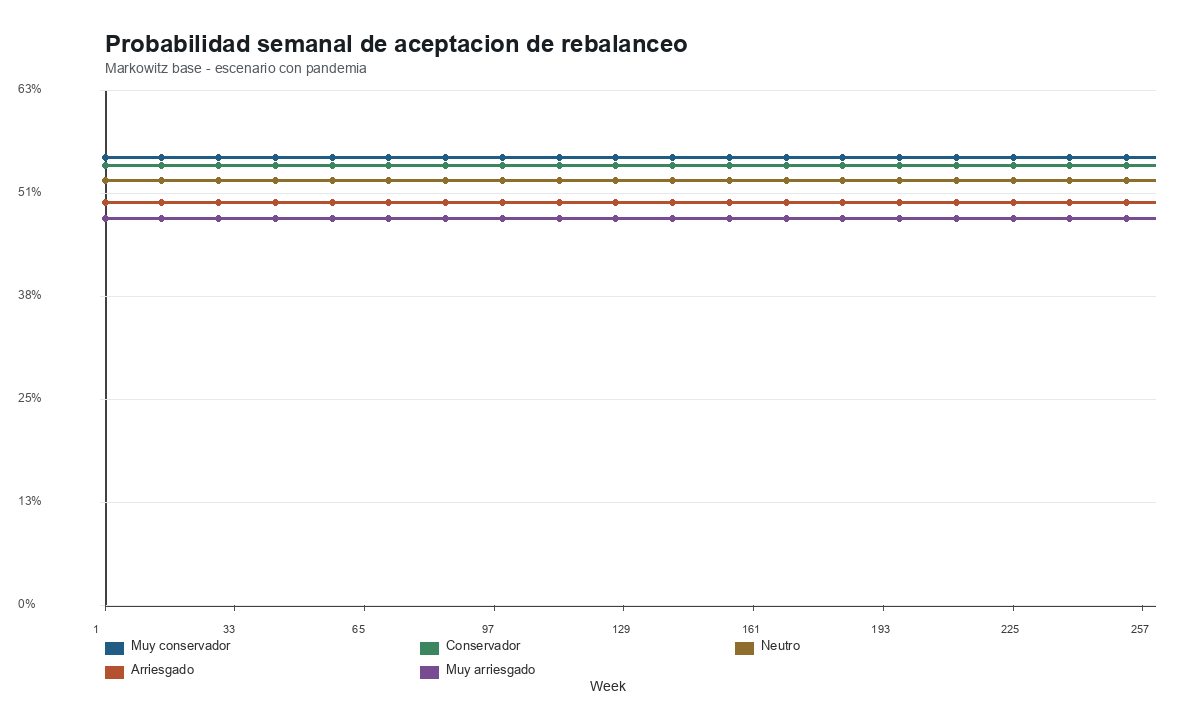
\includegraphics[width=0.92\textwidth]{figuras/aceptacion_weekly_con_pandemia_markowitz_base.png}
\caption{Probabilidad semanal de aceptacion de rebalanceo por perfil, Markowitz base, escenario con pandemia.}
\label{fig:aceptacion_weekly_momentum_general_v1_plus_con_pandemia_markowitz_base}
\end{figure}


\begin{figure}[H]
\centering

\includegraphics[width=0.92\textwidth]{figuras/ganancia_weekly_con_pandemia_markowitz_base.png}
\caption{Ganancia semanal promedio por perfil, Markowitz base, escenario con pandemia.}
\label{fig:ganancia_weekly_momentum_general_v1_plus_con_pandemia_markowitz_base}
\end{figure}


\begin{figure}[H]
\centering

\includegraphics[width=0.92\textwidth]{figuras/clientes_monthly_con_pandemia_markowitz_base.png}
\caption{Clientes activos mensuales por perfil, Markowitz base, escenario con pandemia.}
\label{fig:clientes_monthly_momentum_general_v1_plus_con_pandemia_markowitz_base}
\end{figure}


\begin{figure}[H]
\centering

\includegraphics[width=0.92\textwidth]{figuras/abandono_monthly_con_pandemia_markowitz_base.png}
\caption{Probabilidad mensual de abandono por perfil, Markowitz base, escenario con pandemia.}
\label{fig:abandono_monthly_momentum_general_v1_plus_con_pandemia_markowitz_base}
\end{figure}


\begin{figure}[H]
\centering
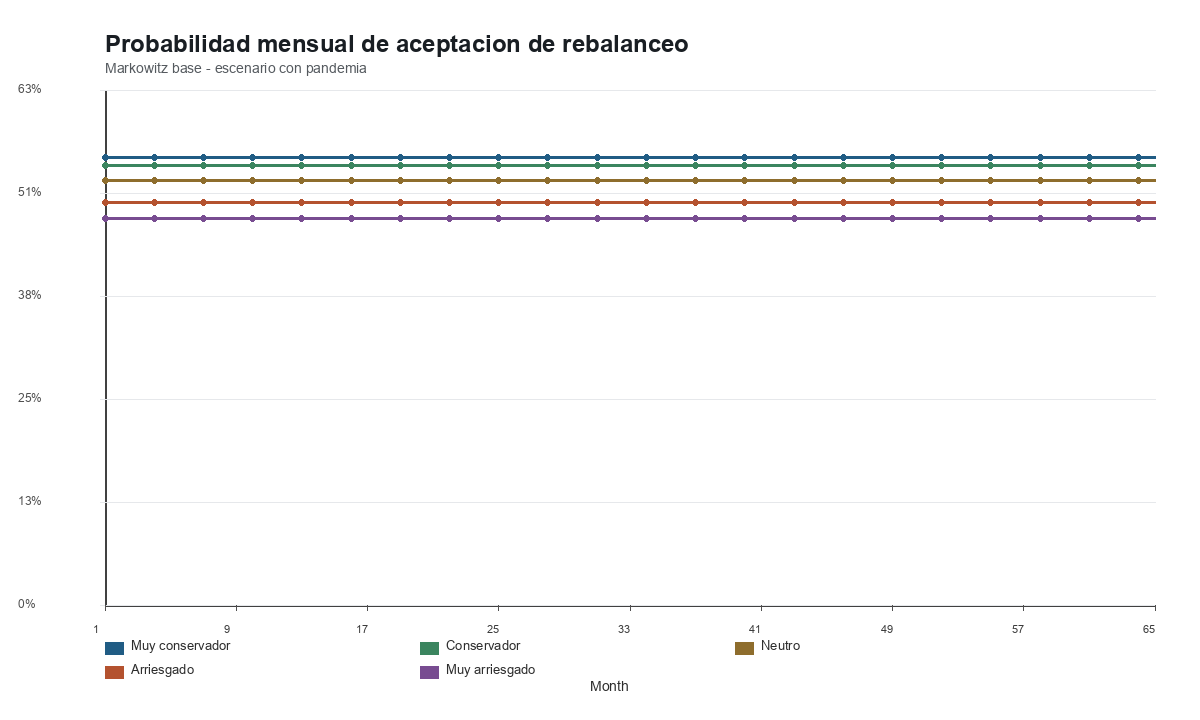
\includegraphics[width=0.92\textwidth]{figuras/aceptacion_monthly_con_pandemia_markowitz_base.png}
\caption{Probabilidad mensual de aceptacion de rebalanceo por perfil, Markowitz base, escenario con pandemia.}
\label{fig:aceptacion_monthly_momentum_general_v1_plus_con_pandemia_markowitz_base}
\end{figure}


\begin{figure}[H]
\centering

\includegraphics[width=0.92\textwidth]{figuras/ganancia_monthly_con_pandemia_markowitz_base.png}
\caption{Ganancia mensual promedio por perfil, Markowitz base, escenario con pandemia.}
\label{fig:ganancia_monthly_momentum_general_v1_plus_con_pandemia_markowitz_base}
\end{figure}


\begin{figure}[H]
\centering

\includegraphics[width=0.92\textwidth]{figuras/ganancia_semiannual_con_pandemia_markowitz_base.png}
\caption{Ganancia semestral promedio por perfil, Markowitz base, escenario con pandemia.}
\label{fig:ganancia_semiannual_momentum_general_v1_plus_con_pandemia_markowitz_base}
\end{figure}


\section{Discusion de Robustez}

La robustez se evalua comparando la persistencia de clientes, la probabilidad de abandono y la ganancia promedio a traves de escenarios con y sin pandemia. El objetivo no es que una view domine en todas las trayectorias, sino que mantenga una relacion defendible entre retorno, riesgo, permanencia de clientes y estabilidad operativa.

\section{Conclusiones}

La version v1 plus mejora la interpretabilidad del modulo P4 porque separa abandono conductual y ruina economica. La restriccion de ruina evita que un cliente sin capital siga contabilizado como activo, mientras que las trayectorias semanales y mensuales permiten observar si la retencion se explica por ausencia de perdidas, tolerancia del perfil o simplemente por baja volatilidad de corto plazo.

\end{document}